\chapter{Επαλήθευση και ταχύτητα επίλυσης}
\label{chapter:results}

Η επαλήθευση ενός αριθμητικού επιλυτή είναι περίπλοκη διαδικασία, καθώς η ακρίβεια ενός τέτοιου προγράμματος ενδέχεται να ποικίλει έντονα ανάλογα με το πρόβλημα.
Επιπρόσθετα, η σύγκριση με αναλυτικές λύσεις, θεωρητικές προβλέψεις, ή πειραματικά δεδομένα περιπλέκεται από το ότι η ακρίβεια της πρόβλεψης εξαρτάται έντονα από το πλέγμα και την ανάλυσή του.
Όσον αφορά την αριθμητική μέθοδο της εργασίας που είδαμε στο κεφάλαιο \ref{chapter:theory}, ένας ακόμα παράγοντας που επηρεάζει την ακρίβεια είναι η μέθοδος επίλυσης του προβλήματος Riemann πάνω στις ασυνέχειες της προσεγγιστικής λύσης, καθώς διαφορετικές μέθοδοι παρουσιάζουν διαφορετική αριθμητική ακρίβεια \cite{Knight2006, Toro2012}.

Ο σκοπός αυτής της εργασίας δεν είναι η ανάπτυξη μίας καινούργιας αριθμητικής μεθόδου για την επίλυση προβλημάτων ρευστομηχανικής.
Αντίθετα, είναι η εύρεση ενός τρόπου εύκολου προγραμματισμού τέτοιων αλγορίθμων, χρησιμοποιώντας τα σύγχρονα προγραμματιστικά εργαλεία που είδαμε στο κεφάλαιο \ref{chapter:julia-diffeq}.
Παρόλα αυτά, στο κεφάλαιο αυτό θα δούμε ένα υπολογιστικό πείραμα με τo οποίo επιδυκνείουμε ότι η υλοποίηση της μεθόδου FVM πρώτης τάξης σε συνδιασμό με την μέθοδο AUFS για τον υπολογισμό των ροών που παρέχει το πακέτο της εργασίας, είναι ορθή και καταλήγει σε ποιοτικά και αριθμητικά αποτελέσματα των οποίων το σφάλμα σε σχέση με θεωρητικές προβλέψεις και αποτελέσματα άλλων επιλυτών είναι αποδεκτό.

\section{Επαλήθευση}

\subsection{Υπολογισμός συνθηκών κατάντη πλάγιου κρουστικού κύματος}

Στο παράδειγμα αυτό θα προσπαθήσουμε να εκτιμήσουμε τις συνθήκες κατάντη (downstream) ενός πλάγιου κρουστικού κύματος (oblique shock wave).
Η ροή συναντά μία κυρτή γωνία (deflection angle) που στρέφει την ροή κατά γωνία $\theta \approx 11.31 \degree$ προς τα επάνω.
Αυτό οδηγεί στην εμφάνιση πλάγιου κρουστικού κύματος του οποίου τις ιδιότητες μπορούμε να προβλέψουμε από την θεωρία της αεροδυναμικής \cite{Anderson2003}.

Μπορούμε έτσι να κατασκευάσουμε το ακόλουθο υπολογιστικό πείραμα.
Θεωρούμε ότι έχουμε τον χώρο του σχήματος \ref{fig:wedge-geometry}.
Δημιουργούμε 4 πλέγματα διαφορετικής ανάλυσης, και για το καθένα επιλύουμε την ροή για έναν διακριτό αριθμό αριθμών Mach, από Mach 2 έως Mach 5.

\begin{figure}[H]
    \centering
    \begin{tikzpicture}[scale=7]
        \draw (0, 0) -- (0.5, 0) -- (1.5, 0.2) -- (1.5, 1) -- (0, 1) -- cycle;
        \draw[dashed] (0.5, 0) -- (1.5, 0.8);
        \draw (0.1, 0.6) node[below right, align=center] {$M_\infty\in\left[2,5\right]$\\$p_\infty=1$\\$\rho_\infty=1.4$};
        \draw[-{Latex[scale=2]}] (0.1, 0.3) -- (0.4, 0.3);

        \draw[dotted]
            (1.75, 0) coordinate (a)
            -- (0.5, 0) coordinate (b)
            -- (1.75, 0.25) coordinate (c)
            pic["$\theta$", draw=black, <->, angle eccentricity=1.1, angle radius=4cm]
            {angle=a--b--c};

        \draw (1.25, 0.45) node[below, align=center] {$M_2$\\$p_2$, $\rho_2$}; 
        \draw[-{Latex[scale=2]}] (1.1, 0.2) -- (1.4, 0.26);
    \end{tikzpicture}
    \caption{Η γεωμετρία του υπολογιστικού πειράματος για τον υπολογισμό των συνθηκών κατάντη πλάγιου κρουστικού κύματος.}
    \label{fig:wedge-geometry}
\end{figure}

Από την γεωμετρία του προβλήματος, μπορούμε να παράξουμε τα μή δομημένα πλέγματα με τον παρακάτω κώδικα Gmsh:

\begin{samepage}
\begin{lstlisting}[style=jlcodestyle]
Point(1) = {0, 0, 0, 0.02};
Point(2) = {0.5, 0, 0, 0.02};
Point(3) = {1.5, 0.2, 0, 0.02};
Point(4) = {1.5, 1, 0, 0.02};
Point(5) = {0, 1, 0, 0.02};

Line(1) = {1, 2};
Line(2) = {2, 3};
Line(3) = {3, 4};
Line(4) = {4, 5};
Line(5) = {5, 1};

Curve Loop(1) = {1, 2, 3, 4, 5};

Plane Surface(1) = {1};

Physical Curve("inlet") = {5};
Physical Curve("outlet") = {3};
Physical Curve("top") = {4};
Physical Curve("bottom") = {1, 2};

Mesh 2;
\end{lstlisting}
\end{samepage}

ελέγχοντας το μέγεθος (και συνεπώς και τον αριθμό) των στοιχείων με την παράμετρο \texttt{clscale} του προγράμματος.

Εκτελώντας συνολικά $13 \times 4 = 52$ προσομοιώσεις παίρνουμε τα αποτελέσματα των σχημάτων \ref{fig:p-d-ratios} και \ref{fig:grid-conv}.
Παρατηρούμε ότι έχουμε σημαντικά μεγαλύτερο σφάλμα για μεγάλους αριθμούς Mach, γεγονός το οποίο αποδίδουμε σε πιθανώς μεγαλύτερη διάχυση των κυμάτων από την διακριτοποίηση πρώτης τάξης.
Από την σχήμα \ref{fig:grid-conv} βλέπουμε ότι το σφάλμα μειώνεται καθώς αυξάνει η ανάλυση του πλέγματος, γεγονός που μας επιτρέπει να ισχυριστούμε ότι με βάσει αυτές τις παρατηρήσεις, η υλοποίηση του επιλυτή μας δεν είσάγει κάποιο σφάλμα, και μπορούμε να πετύχουμε αυθαίρετη ακρίβεια αυξάνοντας την ανάλυση του πλέγματος, με την εξαίρεση σφαλμάτων που μπορεί να εισάγει το σχήμα AUFS.

\begin{figure}
    \centering
    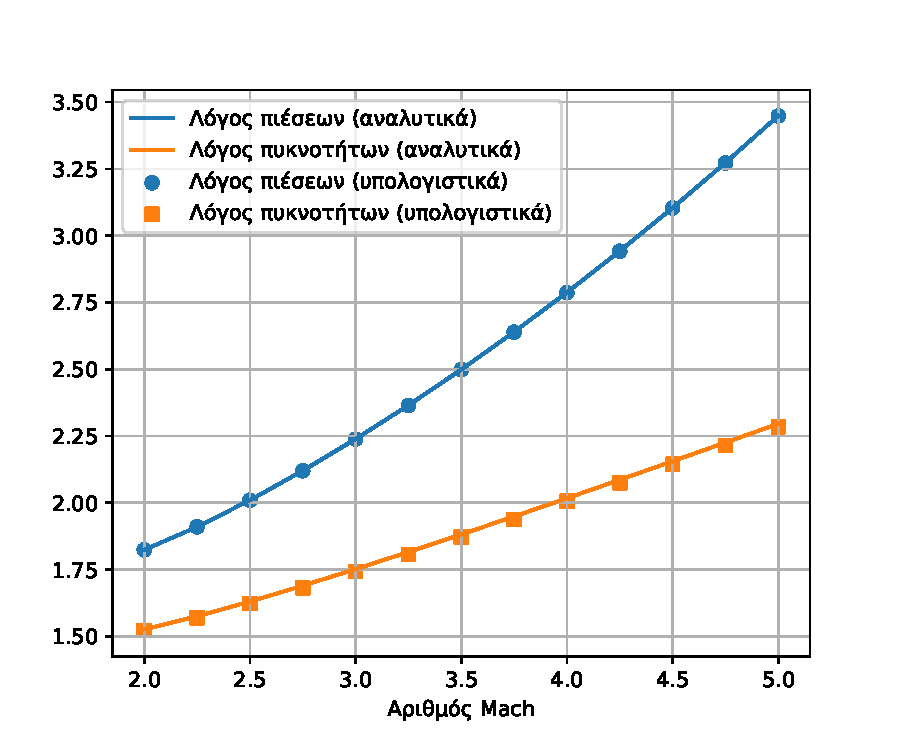
\includegraphics[width=0.7\textwidth]{p-d-ratios}
    \caption{Η εξέλιξη του λόγου πιέσεων και του λόγου πυκνοτήτων σε σχέση με τον αριθμό Mach, σε σύγκριση με την αναλυτική πρόβλεψη, για το πλέγμα με τον μέγιστο αριθμό στοιχείων του πειράματος.}
    \label{fig:p-d-ratios}
\end{figure}

\begin{figure}
    \centering
    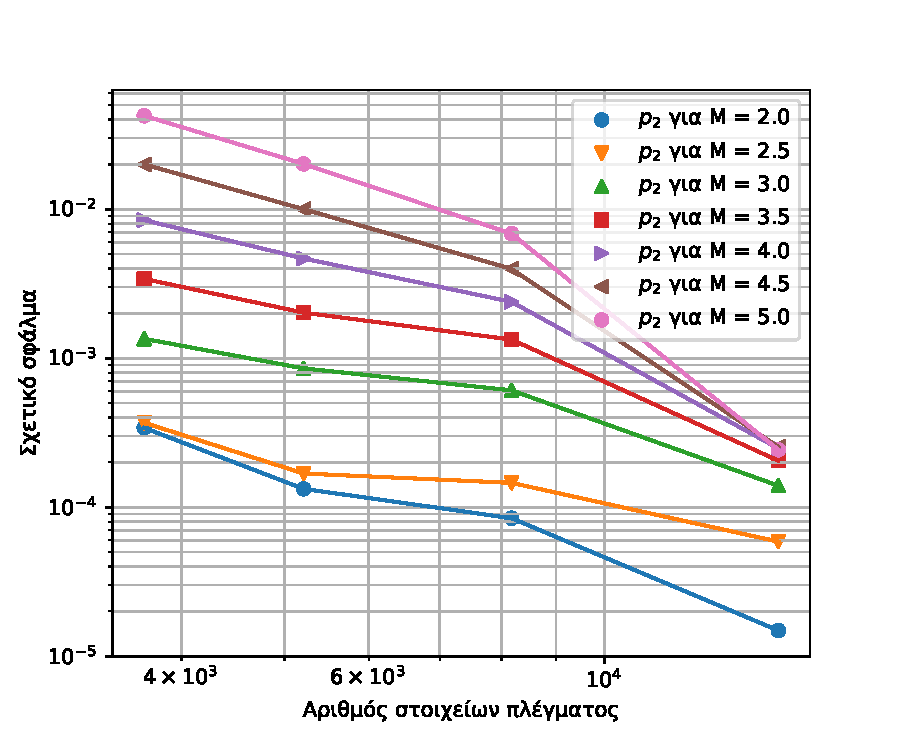
\includegraphics[width=0.7\textwidth]{grid-convergence}
    \caption{Το σχετικό σφάλμα σε σχέση με τον αριθμό στοιχείων του μη δομημένου πλέγματος για τον λόγο πιέσεων από Mach 2 έως Mach 5 σε σύγκριση με την θεωρητική πρόβλεψη.}
    \label{fig:grid-conv}
\end{figure}

% validation

% \subsection{Ροή γύρω από αεροτομή σχήματος ρόμβου}
% 
% Εξετάζουμε επίσης την ροή γύρω από μία αεροτομή σχήματος ρόμβου, το παράδειγμα δηλαδή του κεφαλαίου \ref{chapter:shockwave}, και συγκρίνουμε το αποτέλεσμα του πακέτου μας με αυτό του επιλυτή SU2 \cite{Palacios2013}.
% 
% % diamond -> compare with SU2
% 
% \begin{equation*}
%     d_{r} = \frac{|x - y|}{\max\left(x, y \right)}
% \end{equation*}
% 
% average relative difference mean 0.00844603 / maximum 0.248344 on the leading edge and the shockwaves
% performance

\section{Απόδοση}

Ο κώδικας του πακέτου είναι γραμμένος ακολουθώντας τις προτεινόμενες πρακτικές για κώδικα υψηλής απόδοσης στην Julia.
Η βασικότερη αρχή που ακολουθείται είναι ότι αποφεύγεται η εκχώρηση μνήμης σε κομμάτια κώδικα που εκτελούνται συχνά, όπως π.χ. στο εσωτερικό βρόχων.
Συνεπώς, καθώς η Julia μεταγλωττίζει τον κώδικα μέσω του LLVM, το οποίο με την σειρά του εφαρμόζει μία σειρά από βελτιστοποιήσεις που είναι ανεξάρτητες της γλώσσας υψηλού επιπέδου, η απόδοση του πακέτου μας δεν θα πρέπει να υστερεί σε σχέση με αυτήν των υπόλοιπων επιλυτών παρομοίων προβλημάτων που είναι γραμμένοι σε χαμηλότερου επιπέδου γλώσσες όπως η C++ ή η Fortran.

Ως ένα παράδειγμα της απόδοσης του κώδικά μας, θα εξετάσουμε την ταχύτητα επίλυσης του προβλήματος υπερηχητικής ροής γύρω από αεροτομή σε σχήμα ρόμβου, που είδαμε ως παράδειγμα στο κεφάλαιο \ref{chapter:shockwave}.
Οι μετρήσεις ταχύτητας εκτέλεσης μόνο με CPU έγιναν σε συστήματα της υπολογιστκής συστοιχείας του τμήματος επιστήμης υπολογιστών του πανεπιστημίου Duke, σε υπολογιστικού κόμβους με επεξεργαστές Intel\textregistered  Xeon\textregistered  E5640 με συχνότητα λειτουργίας 2.67 GHz.
Επιπρόσθετα, πραγματοποιήθηκαν μετρήσεις απόδοσης σε κόμβους της ίδιας υπολογιστικής συστοιχείας εφοδιασμένους με κάρτες γραφικών NVIDIA Tesla P100-PCIE με 16 GB μνήμης.

Για να μην διαστρεβλώσουμε τις μετρήσεις με χρόνους που σχετίζονται με είσοδο/έξοδο δεδομένων, μεταγλώττιση πακέτων, και άλλες παράπλευρες εργασίες σταθερού κόστους, αντί να μετρήσουμε τον χρόνο επίλυσης του συνολικού προβλήματος μέχρι την σύγκλιση θα μετρήσουμε τον μέσο χρόνο ανά επανάληψη, δηλαδή τον χρόνο που χρειάζεται για την εκτέλεση ενός χρονικού βήματος.

Τα αποτελέσματα δίνονται στον παρακάτω πίνακα:

\begin{center}
    \begin{tabular}{|c|c|c|c| }
        \hline
        Αρχιτεκτονική & Αριθμός νημάτων & Χρόνος ανά επανάληψη & Επιτάχυνση \\
        \hline
        CPU & 1 & $62.908 \pm 1.080$ ms & 1.0x \\
        CPU & 2 & $35.784 \pm 0.608$ ms & 1.758x \\
        CPU & 4 & $30.431 \pm 0.552$ ms & 2.067x \\
        CPU & 8 & $31.163 \pm 1.256$ ms & 2.019x \\
        \hline
        \multicolumn{2}{|c|}{GPU (CUDA)} & $644.48 \pm 10 $ μs & 97.61x \\
        \hline
    \end{tabular}
\end{center}

Παρατηρούμε ότι για πάνω από 4 νήματα το κόστος από τα παραπάνω νήματα δεν αξίζει τον παραλληλισμό που προσφέρουν, για το συγκεκριμένο πρόβλημα και τον συγκεκριμένο επεξεργαστή.
Εάν ο χρόνος εκτέλεσης παρουσίαζε γραμμική κλιμάκωση με τον αριθμό των νημάτων (που όπως φαίνεται από τον παραπάνω πίνακα, δεν παρουσιάζει), θα χρειαζόταν 97 νήματα για να φτάσουμε τον χρόνο εκτέλεσης που παρουσιάζει η υλοποίηση του επιλυτή για CUDA.

Ως σύγκριση, ρυθμίζοντας τον επιλυτή SU2 έτσι ώστε η μέθοδος επίλυσης να είναι όσο το δυνατόν πιο κοντά στο πακέτο μας, ο μετρούμενος χρόνος είναι περίπου 109.11 ms ανά επανάληψη χρησιμοποιώντας μόνο ένα νήμα.
Αξίζει να τονίσουμε ότι αυτή η σύγκριση δεν είναι πολύ ξεκάθαρη, καθώς το SU2 σχηματίζει τους πεπερασμένους όγκους του γύρω από τις κορυφές των τριγωνικών στοιχείων.
Αυτή η σχεδιαστική επιλογή βοηθάει στο ότι μειώνεται ο αριθμός των όγκων του πλέγματος, αλλά το μειονέκτημα είναι ότι ο κάθε όγκος πλέον μπορεί να έχει διαφορετικό αριθμό γειτόνων.
Αυτό δεν είναι μεγάλο πρόβλημα σε έναν κώδικα που εκτελείται σε παραδοσιακές αρχιτεκτονικές CPU, αλλά κατά την εκτέλεση σε κάρτα γραφικών, κώδικας που δυναμικά πρέπει να χειριστεί τέτοιες περιπτώσεις μπορεί να οδηγήσει σε branch divergence και σημαντική μείωση της απόδοσης \cite{Patterson2017}.
Επιπρόσθετα, η κοντινότερη υπολογιστική μέθοδος που παρέχεται από το SU2 για τον υπολογισμό των ροών είναι η AUSM, η οποία όμως έχει παρόμοιο κόστος υπολογισμού με την AUFS που χρησιμοποιούμε στις παραπάνω μετρήσεις.

\section{Επίλογος}

Το κύριο αποτέλεσμα της εργασίας αυτής είναι ένα καινούργιο πακέτο για την γλώσσα προγραμματισμού Julia, το οποίο επιτρέπει την εύκολη επίλυση προβλημάτων μεταφοράς, προσφέροντας παράλληλα δυνατότητες επιτάχυνσης των υπολογισμών με χρήση καρτών γραφικών που υποστηρίζουν το μοντέλο προγραμματισμού CUDA της NVIDIA.

Αν και το πακέτο της εργασίας είναι μία ικανοποιητική υλοποίηση ως απόδειξη ότι η ανάπτυξη ενός τέτοιου επιλυτή είναι δυνατή, πριν την χρήση του για πραγματικές εφαρμογές χρειάζεται να υλοποιηθεί μία σειρά από δυνατότητες.
Η βασικότερη είναι η υποστήριξη μίας αριθμητικής μεθόδου με ακρίβεια στον χώρο μεγαλύτερη από πρώτη τάξη.
Αν και η μέθοδος πεπερασμένων όγκων μπορεί να επεκταθεί σε δεύτερη ή και μεγαλύτερη τάξη, έχει το πρόβλημα ότι χάνεται η τοπικότητα (locality) στις προσπελάσεις μνήμης, καθώς απαιτείται η προσπέλαση της μνήμης σε στοιχεία μακριά από αυτό στο οποίο θέλουμε να υπολογίσουμε την χρονική παράγωγο.
Αυτό είναι ιδιαίτερα προβληματικό αν μας ενδιαφέρει η εκτέλεση σε κάρτες γραφικών, καθώς για πολλούς αλγορίθμους, ο περιοριστικός παράγοντας για την ταχύτητα του χρόνου εκτέλεσης δεν είναι η ταχύτητα εκτέλεσης των αριθμητικών πράξεων αλλά η ταχύτητα προσπέλασης της μνήμης.
Μία άλλη αριθμητική μέθοδος που πιθανώς ανταποκρίνεται καλύτερα σε αυτό το πρόβλημα είναι η ασυνεχής μέθοδος Galerkin, στην οποία επιλύουμε ένα πρόβλημα πεπερασμένων στοιχείων μέσα σε κάθε πεπερασμένο όγκο.
Η συνάρτηση βάσης $\phi$ δεν χρειάζεται να είναι πλέον σταθερή, και υπάρχουν πολλές επιλογές που μπορούμε να κάνουμε σε αυτό το κομμάτι.
Αυξάνοντας τον αριθμό των συντελεστών της συνάρτησης βάσης, μπορούμε να αυξήσουμε αυθαίρετα την ακρίβεια της χωρικής διακριτοποίησης.
Ενδεχομένως για αυτόν τον λόγο το πακέτο Trixi.jl \cite{Trixi2020} υλοποιεί αυτήν την μέθοδο.

Συνεχίζοντας, χρειάζεται να επεκταθεί η πληθώρα των φυσικών μοντέλων που υποστηρίζει το πακέτο.
Όπως αναφέραμε και παραπάνω, προς το παρόν υποστηρίζεται μονάχα η μέθοδος AUFS.
Υπάρχουν όμως διάφοροι τρόποι υπολογισμού των ροών ανάμεσα στους πεπερασμένους όγκους, με την καθεμία να προσφέρει διαφορετική ακρίβεια και ταχύτητα υπολογισμού \cite{Toro2012}.
Επίσης, η μοντελοποίηση του ιξώδους, το οποίο στην πλειοψηφία των εφαρμογών της αεροδυναμικής δεν μπορούμε να αγνοήσουμε παρά μόνο εάν θέλουμε να πάρουμε μία πολύ γενική εικόνα της ροής, απαιτεί την δυνατότητα επίλυσης εξισώσεων διάχυσης.
Η επίλυση τέτοιων εξισώσεων σε μη δομημένα πλέγματα δεν είναι ιδιαίτερα απλή, καθώς συνήθως απαιτείται ο υπολογισμός ή η εκτίμηση χωρικών παραγώγων, αλλά υπάρχουν μέθοδοι για την επίλυση προβλημάτων διάχυσης σε συνδιασμό τόσο με την ασυνεχή μέθοδο Galerkin όσο και με την μέθοδο πεπερασμένων όγκων.

Ένα άλλο σημαντικό μειονέκτημα της υλοποίησής μας είναι ότι δεν υποστηρίζει εκτέλεση σε διανεμημένα συστήματα, ούτε την χρήση πολλαπλών καρτών γραφικών.
Αυτά τα δύο προβλήματα συνδέονται έντονα, καθώς αναφέρονται στην δυνατότητα εκτέλεσης σε ένα σύστημα που δεν έχει έναν κοινό χώρο μνήμης.
Η συνήθης πρακτική σε τέτοιες περιπτώσεις είναι ο καταμερισμός του πλέγματος σε τμήματα, το καθένα εκ των οποίων ανατίθεται σε έναν υπολογιστικό κόμβο.
Είναι αναγκαία όμως η ανταλλαγή πληροφοριών όσον αφορά τις τιμές της λύσης στα όρια των τμημάτων αυτών, το οποίο απαιτεί την εύρεση αποδοτικών αλγορίθμων ανταλλαγής δεδομένων ανάμεσα στα συστήματα αυτά.
Αν και η υλοποίηση ενός τέτοιου αλγορίθμου είναι περίπλοκη, είναι απαραίτητη για την χρήση του επιλυτή σε προβλήματα μεγάλου μεγέθους τα οποία δεν χωράνε στην μνήμη ενός μεμονωμένου υπολογιστικού κόμβου ή κάρτας γραφικών.

Κλείνοντας, η σημασία αυτού και παρομοίων έργων έχει σημαντικά μεγαλύτερες επεκτάσεις από την μείωση του χρόνου επίλυσης ενός στενού εύρους προβλημάτων με χρήση επιταχυντών όπως είναι οι κάρτες γραφικών.
Αντίθετα, αντιπροσωπεύει έναν τρόπο επίλυσης προβλημάτων υπολογιστικής φυσικής διαφορετικό από το παραδοσιακό μοντέλο των μεγάλων μονολιθικών προγραμμάτων, τα οποία, ακόμη και αν ο πηγαίος κωδικάς τους είναι διαθέσιμος, αποτελούν αυτόνομα συστήματα που δύσκολα συνδιάζονται με άλλους αριθμητικούς αλγορίθμους, ειδικά χωρίς μεγάλες απώλειες σε ταχύτητα.
Ο τρόπος αυτός είναι η ανάπτυξη ενός ομοιόμορφου και ανοικτού οικοσυστήματος επιστημονικών υπολογισμών, στο οποίο οι αλγόριθμοι επίλυσης τέτοιων προβλημάτων αποτελούν μικρότερα σε έκταση, και ευκολότερα κατανοητά προγράμματα, τα οποία είναι εύκολο να συνδιαστούν μεταξύ τους χωρίς μεγάλες απώλειες ταχύτητας.
Αυτή η προσέγγιση ενθαρρύνει τον πειραματισμό και καθιστά την χρήση περίπλοκων αριθμητικών τεχνικών εύκολη για μία μεγάλη ομάδα χρηστών, απαιτώντας μία σημαντικά ομαλότερη καμπύλη εκμάθησης.
Μία τέτοια αλλαγή δεν είναι πρωτόγνωρη.
Αντίστοιχα εργαλεία έχουν καταστήσει την χρήση τεχνικών μηχανικής μάθησης (machine learning) αξιοθαύμαστα προσιτή, με αποτέλεσμα την γρήγορη άνθηση του πεδίου και της εφαρμογής αυτών των τεχνικών σε ένα τεράστιο φάσμα προβλημάτων.
Ενδεχομένως, αυτό να είναι και το μέλλον των εργαλείων της υπολογιστικής φυσικής.


